\section{Project Management}\label{Project Management} 
    In this section, we'll take look at how we organized the team, a brief risk assesment, and an evaluation of the work process. 
    
    \subsection{Team Organization}\label{Team Organization} 
        [The team structure and roles.]
        
        This section describes in detail how we organize ourselves and how we split roles and tasks among the team members. We have a flat team structure and have shifted our focus accordingly over to team communication. 
    
    \subsubsection{Team Structure}\label{Team Structure}
    We already know each other coming into the project so we have chosen a flat organisational structure, with no intervening levels of management, since all decisions within the team will more or less be made by all the members together either way. Relying on the entire group for decisions will both involve and invest everyone in the project and will work well with our already existing group dynamic.
    \footnote{
        Flat organization structure is a structure with few or no levels of intervening management. The idea is that well-trained workers will be more productive when they are directly involved with decision making. 
        [\href{http://en.wikipedia.org/wiki/Flat_organization}{Wikipedia: Flat Ogranization Structure}] 
    }
    
    \begin{figure}[h]
        \centering
        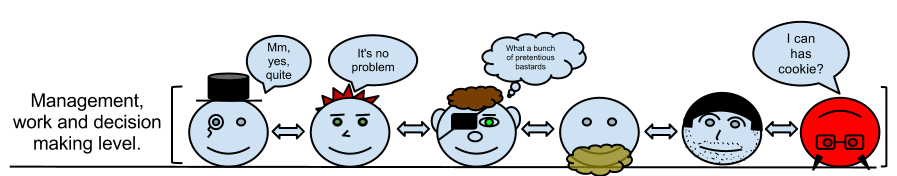
\includegraphics[scale=0.5]{TeamOrganizationchart}
        \caption{Team Organization chart}
        It was made during lunch, but the general principle still remains, that the structure is flat.
        \label{fig:TeamOrganizationchart}
    \end{figure}
    
    %Why changing roles does not work in our structure and how we solve the challenges that might occur in this association. 
    As the structure shows in the chart, there is no difference in what responsibility level anyone have, or what role one has. The concept of changing roles weekly is good for a learning situation, but very inefficient where knowledge and research are key components in a limited timed project. We anticipate that the time for this project probably won't be sufficient for any role changes, and therefore we have to keep people focused on the task they have been assigned. The efficiency of the current task relies on having the current research fresh in mind. If we were to change the roles every week, the newly assigned person would spend much time getting up to date at the beginning of every week, which in turn wouldn't yield any measurable gains. 
    
    Rather than focus on responsibilities within the group, we've chosen to focus on tasks.
The task will to some degree still represent areas of responibilities, and since tasks will be spread across several group members, we don't run the risk of  a single missing member crippling the entire group. Instead the remaining member$($assigned$)$ to a task will be able to pick of the slack. This, together with thorough documentation of a members knowledge, will just about eliminate the problems associated with an absent group member.
        
    Further, the team structure and the distribution of responsibility gives us the chance to define how we want to deal with task and their priority. The work flow that we have makes us prioritise tasks continuously and get the most pressing task done at the correct time. It's similar to a max heap. We put tasks in to the heap, heapify(prioritise tasks) and choose(pop) the maximized task, the task that has the highest priority. 
    
    %Task division and delegation.
    When we choose a task we consider the persons interest, experience and existing knowledge. Most times the tasks fall naturally to one person that has worked with similar tasks earlier in the project. Other times there is more of lottery, where the task has no prerequisites. Often we rely on a persons initiative to take a task or we easily delegate them with a question, "Can someone do that?". Task delegation and sharing the work load has not been a problem so far in the project.
    
    %benefits of a flat team structure. Not very important. 
    
    \subsubsection{Team communication}\label{Team communication}
    We decided that we will work together from 10 to 16, Monday through Thursday every week, with allowed exceptions for lectures and such. Group members can also work in their free time to make up for missed collaboration hours or to just put in some extra work. This means more work than the course requires, but we decided that we want to do it this way so we can either take some time off now and then, or have more time for the exams in May.

    We will not be able to have frequent face to face meetings with the customer, but we will have weekly online meetings with them instead, as well as e-mail communication as needed. Since we have seen what happens in projects where there is little to no communication, we decided, in agreement with the costumer, that we at least wanted to have weekly meetings in order to keep a good dialog with the customer, and also give them the opportunity to take part in the development of the project. Because the customer is located in Oslo, we decided that the weekly meetings will be held over Skype.
    
    \subsection{Risk Assesment}\label{Risk Assesment}
    
    \subsection{Process Evaluation}\label{Process Evaluation}
    % Write something about the fact that we use one day a week to work with planning and paperwork. 
    
    Project management documented: 
    Possible deviations and how they have
been handled. 

    \subsection{Progress tracking and Documentation}\label{Progress tracking and Documentation}
    In the beginning we had a summary every day where we wrote what we were working on and what had to be done. We stopped doing this after we got good activity plans because the daily summaries became unnecessary. 
    
    \begin{figure}[h]
        \centering
        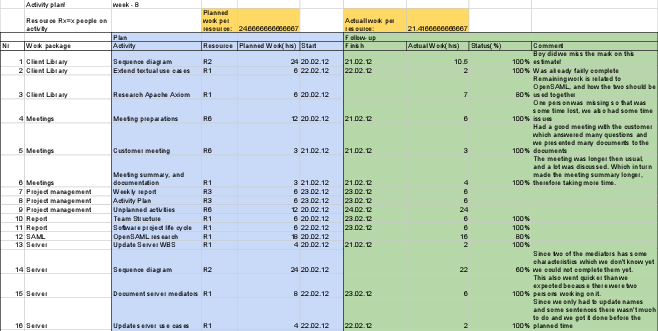
\includegraphics[scale=0.5]{Week8activityplan}
        \caption{Example Activity plan}
        \label{fig:Week8activityplan}
    \end{figure}
    
    The activity plans(Fig:\ref{fig:Week8activityplan}) now have the role of our day to day summaries and work progress. We update the activity plan as we go along. This way we have a complete overview of tasks and work hours that are planned this week. As we update the activity plan we have an overview of the work done this week and where we have missed with our time estimation. 
    
    \begin{figure}[h]
        \centering
        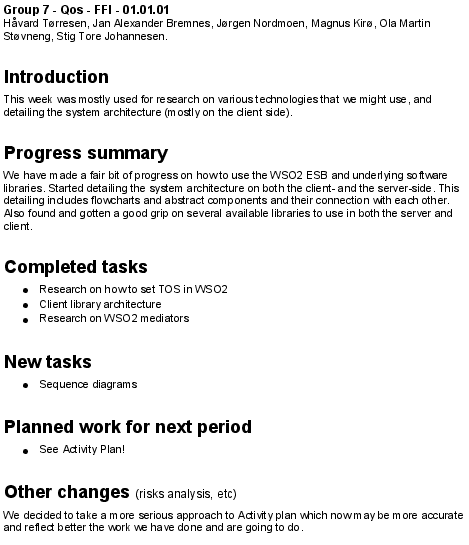
\includegraphics[scale=0.5]{Week7statusreport}
        \caption{Status report example}
        \label{fig:Week7statusreport}
    \end{figure}
    
    As we can se in the weekly report (Fig:\ref{fig:Week7statusreport}) the staus report ha a standard setup. We created a template early in the project so that we did not have to redo the work later. In the prosess of creating the template we put some thought in to it so that we would get a template that would work throughout the project without further changes. 
    
    % write description    

    
    The activity plan has a template which we clone every week to create the plan for next week. We update it  






